%%%%%%%%%%%%%%%%%%%%%%%%%%%%%%%%%%%%%%
% LaTeX poster template
% Created by Nathaniel Johnston
% August 2009
% http://www.nathanieljohnston.com/2009/08/latex-poster-template/
%%%%%%%%%%%%%%%%%%%%%%%%%%%%%%%%%%%%%%

\documentclass[final]{beamer}
\usepackage[scale=1.24]{beamerposter}
\usepackage{graphicx}% allows us to import images
% \usepackage{sidecap}
% \usepackage{sidecap}
\usepackage{wrapfig}
% \usepackage{caption} %removed the figure numbers for some reason?
\usepackage[noabbrev]{cleveref} %add option [capitalize]?
% \usepackage{subfig}
% \usepackage{natbib}


%-----------------------------------------------------------
% Define the column width and poster size
% To set effective sepwid, onecolwid and twocolwid values, first choose how many columns you want and how much separation you want between columns
% The separation I chose is 0.024 and I want 4 columns
% Then set onecolwid to be (1-(4+1)*0.024)/4 = 0.22
% Set twocolwid to be 2*onecolwid + sepwid = 0.464
%-----------------------------------------------------------

\newlength{\sepwid}
\newlength{\onecolwid}
\newlength{\twocolwid}
\newlength{\threecolwid}

\setlength{\paperwidth}{44in}%{48in}{44in}
\setlength{\paperheight}{35in}%{36in}{33in}
\setlength{\sepwid}{0.024\paperwidth}%should be 0.024
\setlength{\onecolwid}{0.22\paperwidth}%should be 0.22
\setlength{\twocolwid}{0.464\paperwidth}%should be 0.464
\setlength{\threecolwid}{0.708\paperwidth}
\setlength{\topmargin}{-0.5in}
\usetheme{confposter}
\usepackage{exscale}

%-----------------------------------------------------------
% The next part fixes a problem with figure numbering. Thanks Nishan!
% When including a figure in your poster, be sure that the commands are typed in the following order:
% \begin{figure}
% \includegraphics[...]{...}
% \caption{...}
% \end{figure}
% That is, put the \caption after the \includegraphics
%-----------------------------------------------------------

\usecaptiontemplate{
\small
\structure{\insertcaptionname~\insertcaptionnumber:}
\insertcaption}

%-----------------------------------------------------------
% Define colours (see beamerthemeconfposter.sty to change these colour definitions)
%-----------------------------------------------------------

\setbeamercolor{block title}{fg=dblue,bg=white}
\setbeamercolor{block body}{fg=black,bg=white}
\setbeamercolor{block alerted title}{fg=white,bg=dblue!70}
\setbeamercolor{block alerted body}{fg=black,bg=dblue!10}

\setbeamercolor{item}{fg=dblue}
\setbeamercolor{item projected}{fg=white,bg=dblue}

%-----------------------------------------------------------
% Name and authors of poster/paper/research
%-----------------------------------------------------------

\newcommand{\sn}{SNIa}

\title{Correlations Between Hubble Residuals and\\\vskip1ex Local Stellar Populations 
of Type Ia Supernovae} 
\author{Benjamin Rose \& Peter Garnavich}
\institute{Department of Physics, University of Notre Dame, Notre Dame, IN 46556\\ \vskip1ex 
brose3@nd.edu}% ~~~ 574.387.3453}

%-----------------------------------------------------------
% Start the poster itself
%-----------------------------------------------------------

\begin{document}
\begin{frame}[t]
\begin{columns}[t]

\begin{column}{\sepwid}\end{column}

\begin{column}{\onecolwid} \label{col1}
\begin{alertblock}{The Big Question}
% What information about Type Ia supernovae will allow us to reduce the scatter on the Hubble diagram?\\
% For Type Ia supernovae to be standard candles their variabilities need to be understood and corrected. 
% In order to improve distance measurements, how can Type Ia supernovae variabilities be better understood and the scatter on the Hubble diagram reduced?
Can using information about the local environment reduce systematic
distance uncertainties in Type Ia supernovae?
\end{alertblock}

% \vskip1ex
%todo:emphaize luminosity-decline rate, color, $x_1$, host galaxy mass, global mentality, and local H$_\alpha$
% \begin{block}{Basic SNIa standardization}
% 
% \end{block}

\vskip1ex

\begin{block}{Environmental Effects}
Type Ia supernovae (\sn{}) are excellent distance indicators, but their Hubble residuals show some correlation with host galaxy properties. 
% Type Ia supernovae (SNIa) are used as a standard candle to measure cosmological distances. 
Each individual \sn{} has some variability, but these can be standardized. The two most popular light curve fitters take into account relationships like luminosity-decline rate %\cite{Phillips93}
and \sn{} color. 
Research over the past several years is indicating that external variables seem to also contribute to \sn{} variability. There are still uncertainties about how the host galaxy and the local environment influence the luminosity, color, and Hubble residuals of \sn{}. 
%These global trends have been researched including metallicity \cite{Hayden13}, and host mass \cite{Childress13}. Other?
%2013ge is one of three from Childress that year.
%Local effects have also been lookedAnd something else about local effect, $H_\alpha$ x2 \cite{Rigault13,Rigault14}. 
There has been research that show the effects of host galaxy mass \cite{Childress13}, global metallicity \cite{Hayden13}, and local H$_\alpha$ \cite{Rigault13}%Rigault14}.

% \vskip1ex
% \begin{itemize}
%     \item global metallicity \cite{Hayden13}
%     \item host galaxy mass (mass step) \cite{Childress13}
%     \item local H$_\alpha$ x2 \cite{Rigault13,Rigault14}
% \end{itemize}
% \vskip1ex
\end{block}

\vskip1ex

\begin{block}{Data Collection}

\begin{itemize}
    \item \sn{} selection, parameters, and cosmology from Campbell (spectroscopic and photometrically classified) \cite{Campbell13}
    \item Local enviorment {\it ugriz} photometry form Holtzman Scene Modeling Photometry \cite{Holtzman08}
    \item Local stellar population model using Conroy's Flexible Stellar Population Synthesis (FSPS, \cite{FSPS1, FSPS2}) and Foreman-Mackey's pyFSPS \cite{pyFSPS}
\end{itemize}

\end{block}

\vskip1ex

\begin{block}{Analysis}
This analysis follows the work of Gupta \cite{Gupta11} but rather then using the \textit{ugriz} of the host from DR7 Stripe 82 co-added catalog we use the local values from Holtzman.
\end{block}
\end{column}


\begin{column}{\sepwid}\end{column}\label{leftspace}


% \begin{column}{\twocolwid}\label{col2}
% \begin{block}{Analysis}
% This analysis follows the work of Gupta \cite{Gupta11} but rather then using the \textit{ugriz} of the host from DR7 Stripe 82 co-added catalog we use the local values at the \sn{} from Holtzman.
% \end{block}

% \vskip1ex

% \begin{columns}
\begin{column}{\onecolwid}
\begin{block}{Stellar Model Parameters}
% This talks about why I chose the model space I did. 

The local stellar population is modeled by a four parameter ``$\tau$-model'', where $\text{SFR} \propto e^{-t/\tau_{\text{SF}}}$. 


\begin{itemize}
    \item $\tau_{\text{SF}}$ -- the e-folding timescale of star formation
    \item $t_{\text{SF}}$ -- the start time for star formation
    \item $\log(Z/Z_{\odot}$) -- the metalicity of the local stellar population
    \item $\tau_{\text{dust}}$ -- the optical depth of the dust around starts older then $7~\text{Gyr}$, younger stars have 3 times the optical depth
\end{itemize}
% Where $\tau_{\text{SF}}$ is the e-folding timescale. This star formation turns on at $t_{\text{SF start}}$. 

% This model also contains changing metalicity and  talk about dust model.

% Details about the values for each parameter are available in table, \Cref{tab:fsps-param}.
\vskip-1ex
\begin{table}[]
    \centering
    \begin{tabular}{c c}
    \hline
    \hline
     FSPS Parameters    & Grid Values \\
    \hline
     $\tau_{\text{SF}}$ [Gyr] & 0.1, 0.5, 1, 2, 3, 4, 6, 8, 10 \\
     $t_{\text{SF}}$ [Gyr] & 0, 1, 2, 3, 4, 5, 6, 7 \\
     $\log(Z/Z_{\odot}$)    & -0.88, -0.59, -0.39, -0.20, 0, 0.20 \\
     $\tau_{\text{dust}}$ & 0, 0.1, 0.3, 0.5, 1.0, 1.5 \\
    \hline
    \end{tabular}
    \caption{FSPS Model Grid Parameters}
    \label{tab:fsps-param}
\end{table}

% These parameters can create a diverse model space as seen in \cref{fig:diverse}.

\begin{figure}
    \begin{minipage}[c]{0.55\onecolwid}
        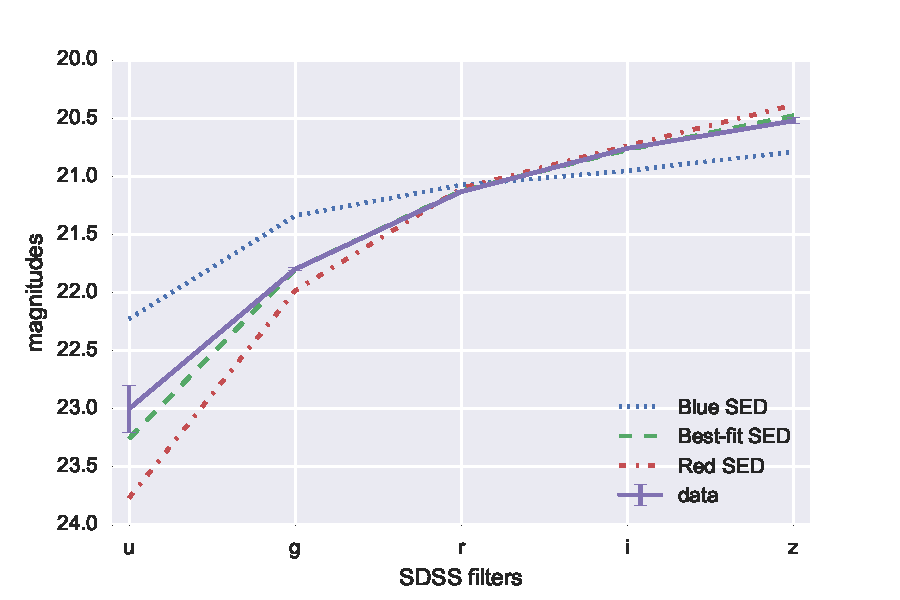
\includegraphics[width=0.67\onecolwid]{SN6057-Model-Variability.pdf}
    \end{minipage}\hfill
    \begin{minipage}[c]{0.35\onecolwid}
    \caption{This figure shows the range of variability of models for SDSS SN6057 (SN 2005if).} \label{fig:diverse}
  \end{minipage}
    % \centering
    % \includegraphics[width=\onecolwid*.95]{SN6057 Model Variability.pdf}
    % 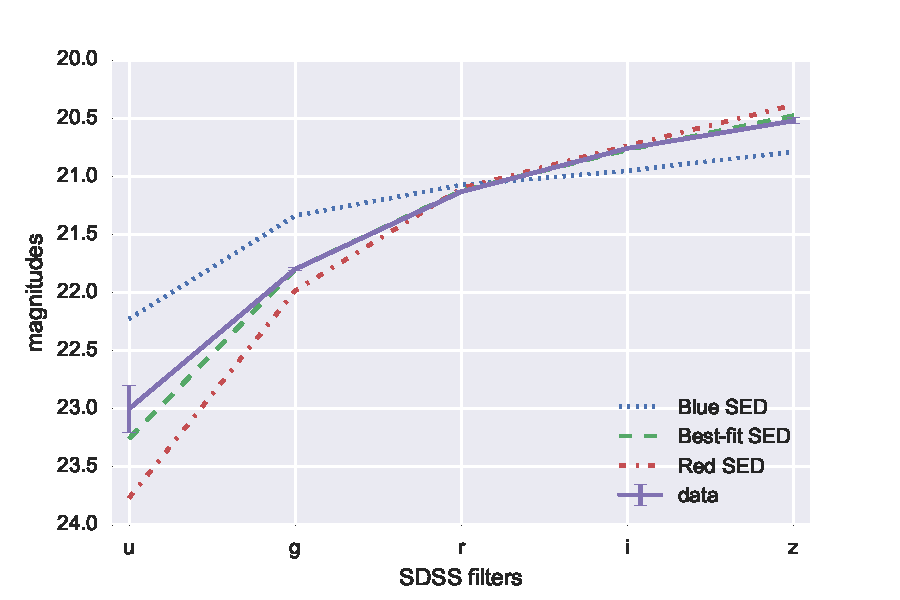
\includegraphics[height=5.5in]{SN6057-Model-Variability.pdf}
    %% 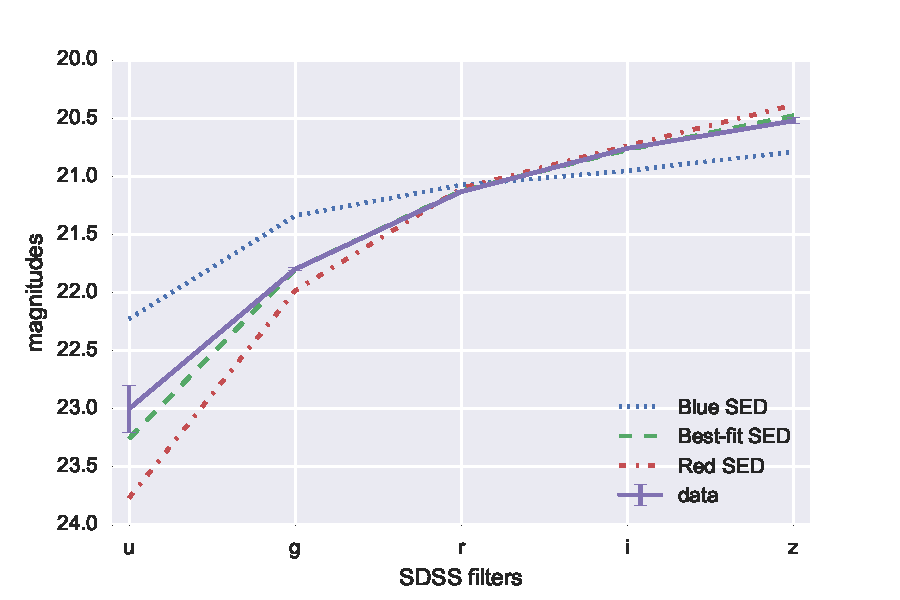
\includegraphics[height=4in]{SN6057-Model-Variability.pdf}
    % 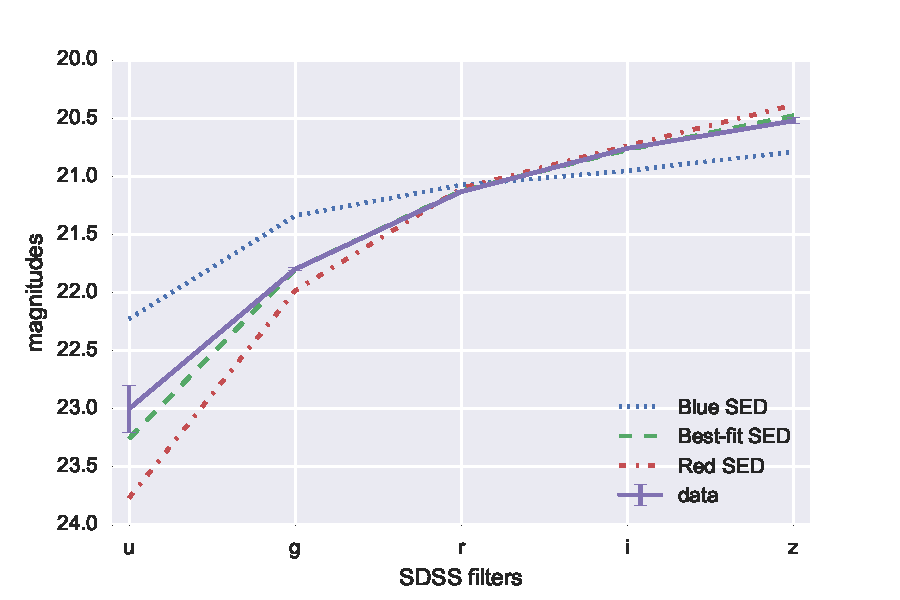
\includegraphics[width=9in]{SN6057-Model-Variability.pdf}
    % \caption{This shows the a the variability of models for SDSS SN6057 (SN 2005if).}
    % \label{fig:diverse}
\end{figure}

\begin{block}{Calculating Local Stellar Age}
The ``best-fit'' model was selected as the one with the lowest $\chi^2$. From this, we calculate the mass weighted age via:
\begin{equation}
    \langle A \rangle_{\text{mass}}= A_{\text{SF}} - \frac{\int^{A_{\text{SF}}}_{0}t\Psi(t)dt}{\int^{A_{\text{SF}}}_{0}\Psi(t)dt}
\end{equation}
Where $A_{\text{SF}}$ is the age of the universe at the given redshift minus $t_{\text{SF}}$ and $\Psi(t)$ is the SFR as a function of time.
% \vskip1ex
Uncertainties were calculated by taking the RMS of the neighboring (in model space) ages scaled by probability of the fit. This results in the equation:
\begin{equation}
    % \sigma_{\text{Age}} = \sqrt[4]{\prod_{i}^{4}\frac{\Delta \text{Age}_i}{\Delta \text{GoF}_i}}
    \sigma_{\text{Age}_{i}} = \frac{e^{-5/2}}{e^{-\chi^2/2}} \sqrt{\langle \Delta \text{Age}_i^2\rangle}
\end{equation}
\end{block}


\end{block}
\end{column}

\begin{column}{\sepwid}\end{column}\label{centerspace}

\begin{column}{\onecolwid}
% \begin{alertblock}{}%{Hubble Residual vs\\Local Stellar Age}
% \begin{figure}
%     \centering
%     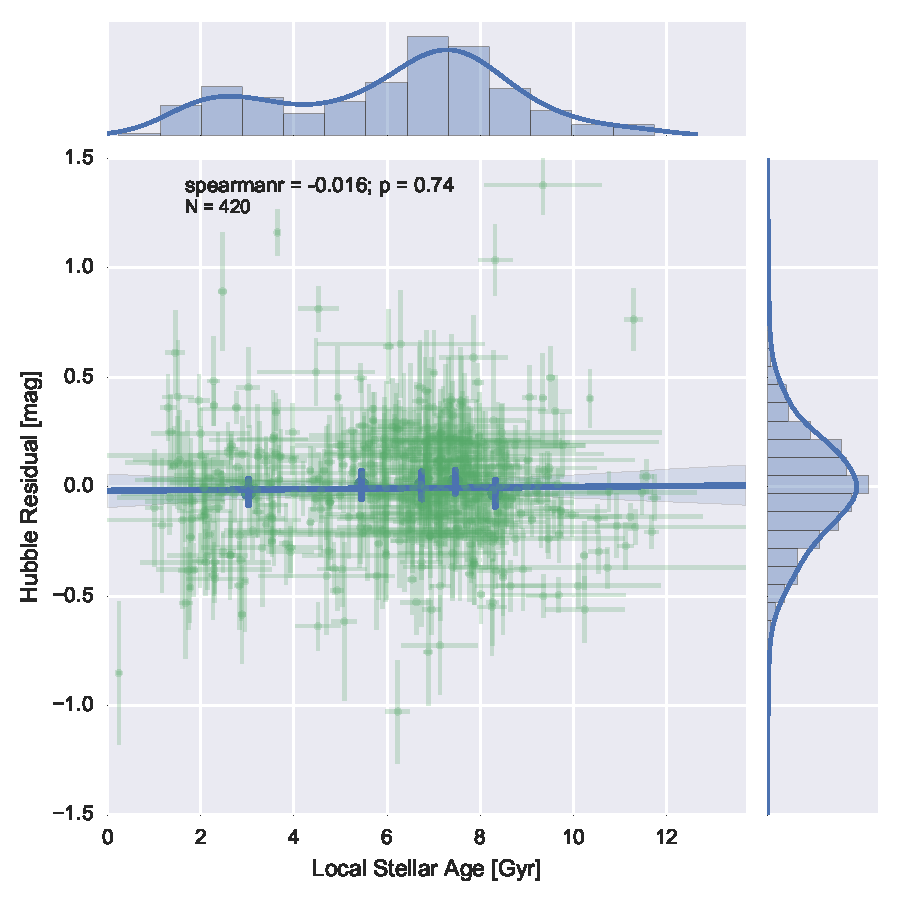
\includegraphics[height=9in]{HRvAge.pdf}
%     % 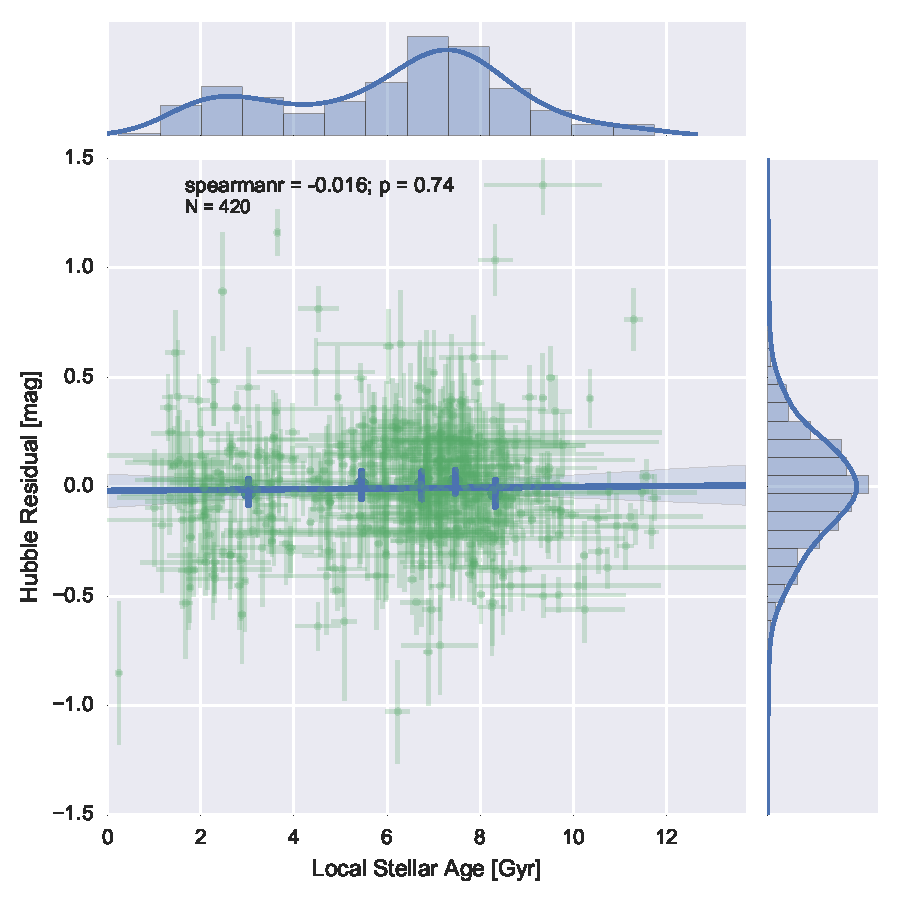
\includegraphics[height=9.5in]{HRvAge.pdf}
%     \caption{There is no correlation between Hubble Residual \cite{Campbell13} and local stellar age as calcualted via FSPS.}
%     \label{fig:HRvAge}
% \end{figure}
% \end{alertblock}

% \vskip1ex

\begin{block}{Local Properties Compared to Hubble Residual}
The Hubble residuals were calculated using Campbell's $\Lambda$CDM best fit: $\text{H}_{0}=73.8~\text{km s}^{-1}~\text{Mpc}^{-1}$, $\Omega_{\text{m}}=0.24$. The results of the Hubble residual versus local stellar population age is seen in \cref{fig:HRvAge}.

% \vskip1ex

\begin{figure}
    \centering
    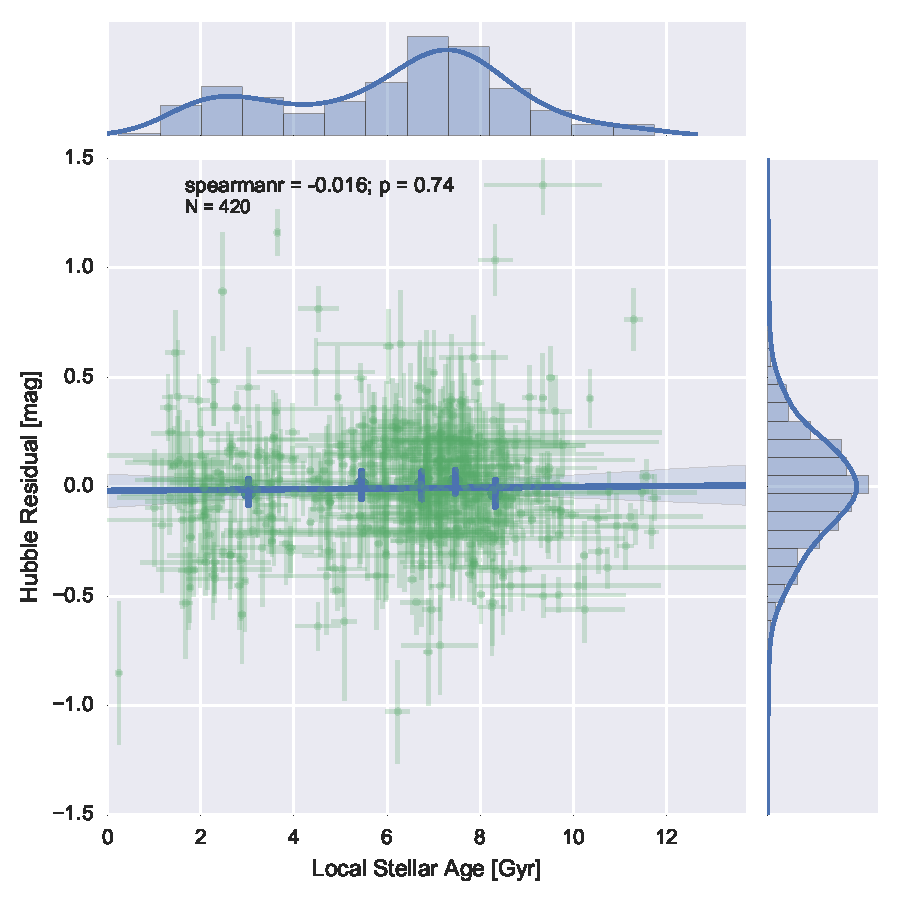
\includegraphics[height=9in]{HRvAge.pdf}
    % 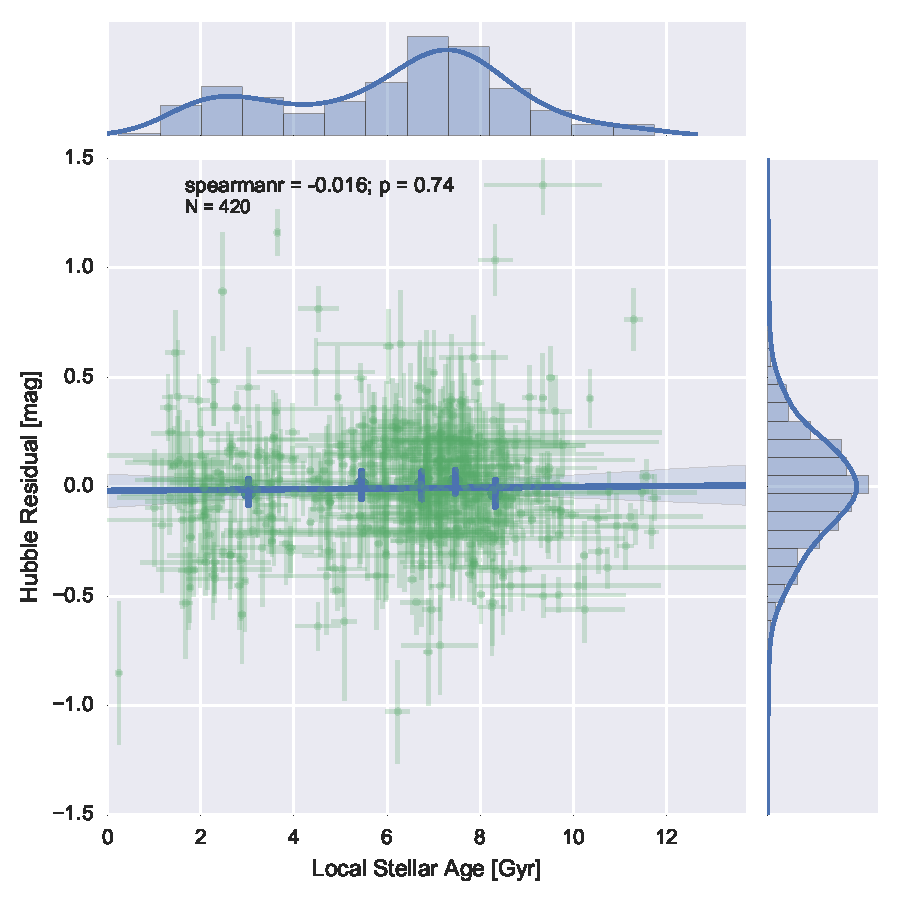
\includegraphics[height=9.5in]{HRvAge.pdf}
    \vskip-0.75ex
    \caption{A linear fit was performed to look for a correlation between Hubble residual and local stellar age: plotted as the blue line. Five binned points (blue) are plotted on top of the complete data set (N=420, green) to guide the eye. 
    % The age population appears to have two clumps at $\sim2~\text{Gyr}$ and $\sim 7~\text{Gyr}$.
    }
    \label{fig:HRvAge}
\end{figure}

\vskip-1.75ex

\begin{figure}
    \centering
    % 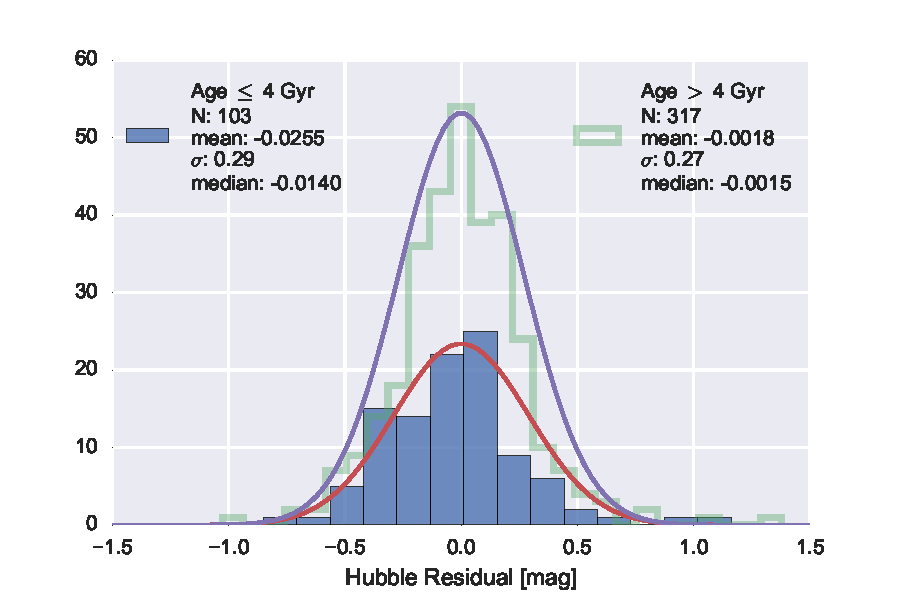
\includegraphics[height=6.5in]{HR_double_hist.pdf}
    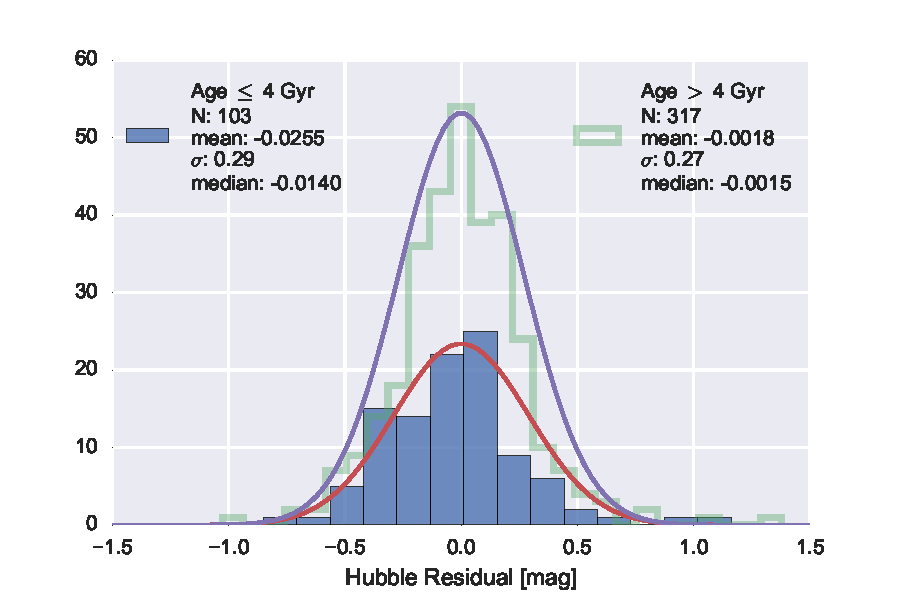
\includegraphics[width=9in]{HR_double_hist.pdf}
    \vskip-0.75ex
    \caption{The distributions of the Hubble residuals split by age. The old population ($> 4~\text{Gyr}$) has a strong Gaussian shape. The young population ($\le 4~\text{Gyr}$) does not appear to have a Gaussian shape but rather a positive skew. The plotted Gaussian (red line) is centered at $0$ with the same $\sigma$ as the old population.}
    \label{fig:HR_hist}
\end{figure}
\end{block}

% "My thought is that the "old" population may just be dominated by background/foreground
% stars unrelated to the supernova...but the young pop are probably associated
% with the supernova (a prompt supernova)." -- Peter

\end{column}


\begin{column}{\sepwid}\end{column}\label{rightspace}


\begin{column}{\onecolwid}\label{col3}

\begin{block}{Preliminary Results}
\begin{itemize}
    \item The  local environments divide into two ages: a ``young'' stellar population with ages less than $4~\text{Gyr}$ and an older population.
    \item There is no clear trend of Hubble residual with local stellar age.
    \item The young population appears to have a non-Gaussian distribution of Hubble residual that may suggest a mix of progenitors similar to Rigault \cite{Rigault13}.
    % \item Rigault \cite{Rigault13} finds a mix progenitor model, and at first glance my results are similar.
    \item There appears to be a difference between local age and global age, Gupta \cite{Gupta11} does not have a bimodal global age distribution.%, but rather a mean of $\sim 4~\text{Gyr}$, in between my two peaks.
\end{itemize}
\end{block}

\vskip1ex

\begin{block}{What is Next}
Investigate differences and similarities between global host parameters and local environment parameters, specifically age distribution. Also investigate a mixed progenitor model to explain the non-Gaussian Hubble residuals of the young stellar population.
\end{block}

\vskip1ex

\begin{block}{References} 
% \bibliographystyle{apj}
%using small, but could also use footnotesize, but other sizes are too small.
\footnotesize{\begin{thebibliography}{99}
% \bibitem{Phillips93}Phillips, M. M. 1993, ApJ, L105, 413
\bibitem{Childress13}Childress, Aldering, Antilogus, et al. 2013, ApJ, 770, 108
%I may want another 
\bibitem{Hayden13}Hayden, Gupta, Garnavich, et al. 2013, ApJ, 764, 191
\bibitem{Rigault13} Rigault, Copin, Aldering, et al. 2013, A\&A, 560, A66
\bibitem{Campbell13} Campbell, D'Andrea, Nichol, et al. 2013. ApJ, 763, 88
\bibitem{Holtzman08} Holtzman, Marriner, Kessler, et al. 2008, AJ, 136, 2306
\bibitem{FSPS1} Conroy, Gunn, \& White 2009, ApJ, 699, 486
\bibitem{FSPS2} Conroy \& Gunn 2010, ApJ, 712, 833
\bibitem{pyFSPS} Foreman-Mackey, Sick, \& Johnson 2014. \url{http://doi.org/10.5281/zenodo.12157}
\bibitem{Gupta11} Gupta, D'Andrea, Sako, et al. 2011. ApJ, 740, 92
% \bibitem{astorpy} Astropy Collaboration, 2013
% \bibitem{Rigault14} Rigault, Aldering, Kowalski, et al. 2015, ApJ, 802, 20 
\end{thebibliography}}
\end{block}

\vskip0.5ex

\begin{block}{Acknowledgments} 
\begin{wrapfigure}{r}{0.45\onecolwid}
    \vspace{-33pt}
    \begin{center}
    \subfloat{
        
\includegraphics[width=4.1in]{ND_mark_black.pdf}
    }
    
    \subfloat{
        
\includegraphics[width=4.1in]{astropy_powered.png}
    }
    \end{center}
\end{wrapfigure}
%using small, but could also use footnotesize, but other sizes are too small.
\footnotesize{
% {\bf NEED TO ADD GSU \& GPS FUNDING!} \\
Funding in part by 
% NASA grant HST-GO-129, 
the Notebaert Professional Development Fund, and ND Graduate Student Union CPG.
\vskip1.5ex
\textit{Software:} 
Astropy, Numpy, Pandas, \\Matplotlib, Seaborn, FSPS, Python-FSPS
}
% \vskip1ex
% \begin{center}
% \begin{tabular}{cc}
%     % \vspace{53pt} 
%     % \vspace*{-20pt}
%     
\includegraphics[width = 4.5in]{ND_mark_black.png} &%$~~~~$&
%     % \vspace{-210pt}
%     
\includegraphics[width = 4.5in]{astropy_powered.png}
% \end{tabular}

% 
\includegraphics[width = 4.5in]{ND_mark_black.pdf}
% % \\ \vskip1ex
% $~~~$
\includegraphics[width = 4.5in]{astropy_powered.png}

% \end{center}

% \begin{figure}
%     \begin{center}
%     % \subfloat{
%         
\includegraphics[height=0.9in]{ND_mark_black.pdf}
%     % }
    
%     % \subfloat{
%         % 
\includegraphics[height=0.8in]{astropy_powered.png}
%     % }
%     \end{center}
% \end{figure}
\end{block}
\end{column}

\begin{column}{\sepwid}\end{column}

\end{columns}
\end{frame}
\end{document}